% !TeX program = lualatex
% !TeX encoding = UTF-8
% !TeX spellcheck = en_US

\documentclass[
    12pt                % Font size
]{article} % Sets the base font size (12pt) and document class (article)

% --- Language and Encoding ---
\usepackage[english]{babel} % Language (adjust if primary language is German)

\usepackage{amsmath}        % For advanced math typesetting
\usepackage{amssymb}        % For math symbols
\usepackage{graphicx}       % For including images
\usepackage{csquotes}       % Context sensitive quotation marks, often needed by biblatex
\usepackage{times}          % Uses Times New Roman font

% --- Bibliography ---
\usepackage[
    backend=biber,        % Use biber backend
    style=apa,            % APA citation style (or another like 'authoryear')
    sorting=nyt,          % Sort by name, year, title
    natbib=true           % Enable natbib compatibility commands if needed
]{biblatex}
\addbibresource{../EV_utils/resources.bib} % Specifies the bibliography file

% --- Hyperlinks and PDF Metadata ---
\usepackage{hyperref} % Enables clickable links within the PDF (e.g., ToC, citations, URLs)
\hypersetup{
    hidelinks, % Hides the borders/colors around links
    colorlinks=true, % Colors the link text instead of using borders
    breaklinks=true, % Allows links to break across lines
    urlcolor=black, % Color for URLs
    citecolor=black, % Color for citation links
    linkcolor=black, % Color for internal links (sections, figures)
    bookmarksopen=false, % Whether PDF bookmarks are initially expanded
    pdftitle={EmotiView: Neural-Autonomic Synchrony in Conscious Emotional Processing}, % PDF metadata: Title
    pdfauthor={Cagatay Özcan Jagiello Gutt} % PDF metadata: Author
}

% --- Graphics and Page Layout ---
\usepackage{geometry} % For customizing page margins and layout
\geometry{a4paper, margin=1in} % Sets paper size to A4 and all margins to 1 inch
\usepackage{float} % Improves control over floating elements like figures and tables

% --- Captions ---
\usepackage{caption}
\captionsetup{
    justification=justified, % Justifies caption text
    singlelinecheck=false, % Applies justification even to single-line captions
    labelfont=bf, % Makes the caption label (e.g., "Figure 1:") bold
    margin=1.5em, % Sets left/right margin for caption text
    font={stretch=1.0} % Adjusts line spacing within captions (1.0 is normal)
}

% --- Diagrams and Drawing ---
\usepackage{tikz} % Powerful package for creating graphics programmatically
\usetikzlibrary{arrows.meta, shapes.geometric, positioning, decorations.pathreplacing} % Loads useful TikZ libraries

% --- Text Formatting ---
\usepackage{ragged2e} % Provides improved text alignment options (e.g., \RaggedRight)
\usepackage{enumitem}
\usepackage{microtype}
\usepackage{setspace} % For adjusting line spacing (\setstretch, \singlespacing, etc.)

% --- Colors ---
\usepackage{xcolor} % Enables the use of colors
\definecolor{rubblue}{RGB}{0,51,160} % Defines a custom color 'rubblue'
\definecolor{rubgrey}{RGB}{153,153,153} % Defines a custom color 'rubgrey'
\definecolor{borot}{RGB}{226,0,26}
\definecolor{Grau}{gray}{0.96}

% --- Section Spacing Customization ---
\usepackage{titlesec} % Allows customization of section headings
\titlespacing*{\section}{0pt}{*1.2}{*0.7} % Adjusts spacing around \section: {left}{before}{after}
\titlespacing*{\subsection}{0pt}{*1.2}{*0.7} % Adjusts spacing around \subsection
\titlespacing*{\paragraph}{0pt}{*1}{*0.5} % Adjusts spacing around \paragraph

% --- Glossaries and Acronyms ---
\usepackage[automake, % Automatically runs makeglossaries if needed
            acronym, % Enables acronym handling
            toc, % Adds glossaries to the Table of Contents
            shortcuts, % Provides shorthand commands like \acs, \acp
            nomain, % Disables the main glossary type if only acronyms are used
            nonumberlist, % Suppresses page numbers in the glossary list
            nopostdot, % Removes the period after descriptions in the list
            nogroupskip % Removes vertical space between letter groups in the list
           ]{glossaries}
\loadglsentries{../EV_utils/EV_glossary.tex} % Path to your glossary definitions
\makeglossaries % Processes the defined glossaries and acronyms

% --- Glossary Formatting ---
\renewcommand*{\glsnamefont}[1]{\textbf{\textit{#1}}} % Formats the acronym name in the list

% --- Header/Footer Setup ---
\usepackage{fancyhdr} % For creating custom headers and footers
\renewcommand{\headrulewidth}{0.4pt} % Sets the thickness of the header rule line
\renewcommand{\footrulewidth}{0.4pt} % Sets the thickness of the footer rule line
\setlength{\headheight}{14.49998pt} % Sets the height reserved for the header
\addtolength{\topmargin}{-2.49998pt} % Adjusts top margin
\setlength{\parindent}{0 cm} % Sets paragraph indentation to zero

% --- Page Style Setup ---
\pagestyle{fancy} % Activates the fancy page style
\fancyhf{} % Clears all existing header and footer fields
\fancyhead[R]{EmotiView: Neural-Autonomic Synchrony} % Thesis title in header (shortened)
\fancyhead[L]{\nouppercase{\leftmark}} % Current section title (lowercase) in top left header
\fancyfoot[C]{-\thepage-} % Page number centered in the footer
\fancyfoot[L]{Cagatay Özcan Jagiello Gutt} % Author name in bottom left footer
\fancyfoot[R]{\href{https://orcid.org/0000-0002-1774-532X}{ORCID: 0000-0002-1774-532X}}
% Title, Author, Date
\title{EmotiView: Neural-Autonomic Synchrony in Conscious Emotional Processing} % Replace with your actual title
\author{Cagatay Özcan Jagiello Gutt} % Replace with your name
\date{\today}

\begin{document}

% --- Title Page ---
\begin{titlepage}
    \begin{center}
        \begin{minipage}{0.2\textwidth}
            
\includegraphics[width=1.5\textwidth]{../EV_images/rub.jpg} % University logo
        \end{minipage}
        \hspace*{\fill}
        \begin{minipage}{0.6\textwidth}
            \hspace*{\fill}\textbf{Ruhr-University Bochum} \\ \hspace*{\fill}\textbf{Faculty of Psychology}
        \end{minipage}

        \vspace{2 cm}
        {\textbf{\large MASTER THESIS}}

        \vspace{0.2cm}
        Submitted in partial fulfillment of the requirements for the degree of Master of Science in Cognitive Science at Ruhr-University Bochum

        \vspace{0.5cm}
        by the student

        \vspace{0.5cm}
        Cagatay Özcan Jagiello Gutt\\
        Student Number: 108022246097

        \vspace{0.5cm}
        Submission Date: \today \\ % Or a specific date
        Examination Period: Summer Semester 2025 % Adjust as needed

        \vspace{0.5cm}
        Thesis Title:

        \vspace{0.2cm}
        \textbf{Neural-Autonomic Synchrony and Embodied Integration}

        \vspace{0.2cm}
        Temporal Binding of Frontal-Parietal Networks and Autonomic Responses in Conscious Emotional Processing

        \vspace{0.5cm}
        \begin{minipage}{0.8\textwidth}
            \begin{tabular}{p{0.4\textwidth} p{0.4\textwidth}}
                1st Supervisor: & Dr. Julian Elias Reiser \\
                & Leibniz Research Centre for Working Environment and Human Factors (IfADo) \\
                & at TU Dortmund, Department of Psychology and Neurosciences\\
                \\
                2nd Supervisor: & Prof. Dr. Dirk Scheele \\
                & Research Department of Neuroscience, Institute of Cognitive Neuroscience, \\
                & Faculty of Psychology, Ruhr-University Bochum \\
            \end{tabular}
        \end{minipage}
        \vspace{\fill}
    \end{center}
\end{titlepage}
\newpage

% Include your abstract - Placed immediately after the title page
\phantomsection % Ensures hyperref links correctly to the Abstract from the ToC
\addcontentsline{toc}{section}{Abstract} % Adds "Abstract" to the Table of Contents
\begin{abstract}
\documentclass[12pt, a4paper]{article}

% --- Language and Encoding ---
\usepackage[utf8]{inputenc}
\usepackage[T1]{fontenc}
\usepackage[english]{babel}

% --- Bibliography (Included for consistency, though not used in abstract) ---
\usepackage[backend=biber, style=apa]{biblatex}
% \addbibresource{resources.bib} % Specify your bibliography file if needed later

% --- Hyperlinks and PDF Metadata ---
\usepackage{hyperref}
\hypersetup{
    hidelinks,
    colorlinks=true,
    breaklinks=true,
    urlcolor=black,
    citecolor=black,
    linkcolor=black,
    bookmarksopen=false,
    pdftitle={Temporal Binding of Brain and Body: Neural-Autonomic Phase Synchrony During Emotional Processing},
    pdfauthor={Cagatay Özcan Jagiello Gutt}
}

% --- Graphics and Page Layout ---
\usepackage{graphicx}
\usepackage{geometry}
\geometry{margin=1in}
\usepackage{float}

% --- Captions (Included for consistency) ---
\usepackage{caption}
\captionsetup{
    justification=justified,
    singlelinecheck=false,
    labelfont=bf,
    margin=1.5em,
    font={stretch=1.0}
}

% --- Diagrams and Drawing (Included for consistency) ---
\usepackage{tikz}
\usetikzlibrary{arrows.meta, shapes.geometric, positioning, decorations.pathreplacing}

% --- Text Formatting ---
\usepackage{ragged2e}
\usepackage{enumitem}

% --- Colors ---
\usepackage{xcolor}
\definecolor{rubblue}{RGB}{0,51,160}
\definecolor{rubgrey}{RGB}{153,153,153}

% --- Font and General Style Packages (from proposal) ---
\usepackage{times}
\usepackage{fancyhdr}
\usepackage{csquotes}
\usepackage{amsmath}
\usepackage{amsfonts}
\usepackage{amssymb}
\usepackage{makecell}
\usepackage{setspace}

% --- Section Spacing Customization (Included for consistency, though no sections here) ---
\usepackage{titlesec}
\titlespacing*{\section}{0pt}{*1.2}{*0.7}
\titlespacing*{\subsection}{0pt}{*1.2}{*0.7}
\titlespacing*{\paragraph}{0pt}{*1}{*0.5}

% --- Glossaries and Acronyms (REMOVED - Not needed for standalone abstract page) ---
% \usepackage[acronym, shortcuts]{glossaries}
% \newacronym{...} ...
% \makeglossaries
% \renewcommand*{\glsnamefont}[1]{\textbf{\textit{#1}}}

% --- Header/Footer Setup (Matching proposal style, NO page number) ---
\renewcommand{\headrulewidth}{0.4pt}
\renewcommand{\footrulewidth}{0.4pt}
\setlength{\headheight}{14.49998pt}
\addtolength{\topmargin}{-2.49998pt}
\setlength{\parindent}{0 cm}

% --- Custom Colors (Copied from proposal) ---
\definecolor{borot}{RGB}{226,0,26}
\definecolor{Grau}{gray}{0.96}

% --- Custom Commands (Copied from proposal) ---
\newcommand{\mt}[2][Grau]{\colorbox{#1}{#2}}
\newcommand{\ts}[1]{\textsl{#1}}
\newcommand{\q}[1]{\glqq #1\grqq}

% --- Page Style Setup (using fancyhdr - matching proposal) ---
\pagestyle{fancy}
\fancyhf{}
\fancyhead[R]{Neural-Autonomic Synchrony and Embodied Integration}
\fancyhead[L]{\nouppercase{\leftmark Abstract}}
\fancyfoot[R]{\href{https://orcid.org/0000-0002-1774-532X}{ORCID: 0000-0002-1774-532X}}

% --- Title, Author, Date Information ---
\title{Neural-Autonomic Synchrony and Embodied Integration}
\author{Cagatay Özcan Jagiello Gutt}
\date{\today}

% --- Start of Document ---
\begin{document}

% --- Title Block Formatting ---
{\bfseries\maketitle}
\thispagestyle{fancy}
\vspace{-2\baselineskip}

% --- Abstract Environment ---
\begin{abstract}
Emotional states are fundamentally embodied, emerging from the dynamic interplay between central neural processing and peripheral physiological adjustments orchestrated by the autonomic nervous system (ANS). While ANS outputs like heart rate variability (HRV) and electrodermal activity (EDA) reflect emotional arousal and valence, understanding the precise temporal coordination between brain activity and these peripheral signals is crucial for elucidating brain-body interactions. This study investigates neural-autonomic phase synchrony during the conscious processing of distinct emotional states (positive, negative, neutral) by quantifying the temporal alignment between cortical and physiological rhythms.
    
We employ a multimodal approach, simultaneously recording high-temporal-resolution electroencephalography (EEG), electrocardiography (ECG) for HRV analysis (specifically Root Mean Square of Successive Differences, RMSSD), EDA, and functional near-infrared spectroscopy (fNIRS) while participants view validated emotional video clips. Our primary analysis quantifies the Phase Locking Value (PLV) between frontal EEG oscillations (Alpha, Beta bands) and continuous signals derived from HRV (reflecting parasympathetic influence) and phasic EDA (reflecting sympathetic influence). EEG channel selection for PLV analysis was informed by task-related hemodynamic activity measured via fNIRS to focus on functionally relevant cortical areas.
    
We hypothesize that PLV, indicating brain-body temporal integration, will be significantly modulated by emotional content compared to neutral conditions. We further expect synchrony strength to correlate with subjective arousal ratings. By examining the phase synchrony between brain signals and ANS-mediated physiological outputs, this research provides novel insights into the dynamic, embodied mechanisms underlying emotional experience. Understanding this temporal binding is critical for models of psychophysiological function and may inform assessments of cognitive load or stress regulation capacity, potentially impacting performance monitoring and optimization in demanding operational environments.
\end{abstract}
    
\end{document}
 % Inserts the content of your abstract file
\end{abstract}
\cleardoublepage % Ensure next content (e.g., ToC) starts on a new page

\pagenumbering{Roman} % Roman numerals for front matter (ToC, LoF, Glossary)

\tableofcontents
\newpage
\listoffigures
% \listoftables % Uncomment if you have tables
\newpage
\printglossary[style=long3col, type=\acronymtype, title=List of Acronyms] % Acronyms list
\newpage
\pagenumbering{arabic} % Arabic numerals for main body

% Include your chapters/sections
% \include{introduction} % Example: create introduction.tex
\section{Methods}

\subsection{Electroencephalography}
\gls{EEG} was used to measure electrical brain activity via scalp electrodes, capturing voltage fluctuations from synchronized postsynaptic potentials primarily in cortical pyramidal neurons \parencite{sharmaEmergingTrendsEEG2024, chaddadElectroencephalographySignalProcessing2023}. Its excellent temporal resolution (milliseconds) was indispensable for capturing the rapid neural dynamics underlying emotional processing and for performing phase synchrony analysis (\gls{PLV}) with concurrently measured physiological signals \parencite{cohenAnalyzingNeuralTime2014}. While its spatial resolution is inherently limited by volume conduction effects, \gls{EEG} allowed for the tracking of oscillatory activity in specific frequency bands that are well-established correlates of cognitive and affective states. Consistent with the literature cited in the introduction, the focus was on the Alpha (8-13 Hz) band, which is not only associated with cortical inhibition and attentional processes but also critically implicated in emotional valence processing, particularly within the context of frontal asymmetry and the motivational direction model \parencite{allenIssuesAssumptionsRoad2004, klimeschEEGAlphaTheta1999}. Additionally, the Beta (13-30 Hz) band was investigated, as it is implicated in active cortical processing, sensorimotor integration, maintaining the current cognitive set, and potentially reflecting arousal states relevant to emotional engagement \parencite{engelDynamicPredictionsOscillations2001, koenigMillisecondMillisecondYear2002}. \gls{EEG} thus provided the primary high-resolution neural signal for assessing frontal asymmetry (via alpha power) and for calculating \gls{PLV} (using phase information extracted from both alpha and beta bands) to investigate brain-body coupling.

\subsection{Functional Near-Infrared Spectroscopy}
\gls{fNIRS} was employed to measure cerebral hemodynamic changes, specifically concentrations of \gls{HbO2} and \gls{HbR}, which are linked to neural activity via neurovascular coupling \parencite{scholkmannReviewContinuousWave2014, jobsisNoninvasiveInfraredMonitoring1977, obrigVisibleImagingHuman2003}. This technique uses near-infrared light to non-invasively monitor changes in blood oxygenation, reflecting the increased metabolic demand and subsequent blood flow adjustments in active brain regions. Offering spatial information complementary to the high temporal resolution of \gls{EEG} \parencite{pintiCurrentStatusIssues2019}, \gls{fNIRS} enabled the localization of sustained hemodynamic correlates of neural activity within specific cortical regions. As outlined in the introduction, a key role of \gls{fNIRS} in this study was to identify prefrontal \gls{ROI} demonstrating significant task-related activation during emotional processing. This functional localization was then used to guide the selection of \gls{EEG} channels for the synchrony analysis, thereby helping to spatially constrain and interpret the functional significance of observed \gls{EEG}-autonomic coupling originating from these emotionally engaged areas.

\subsection{Electrocardiography and Heart Rate Variability}
\gls{ECG} was used to record the heart's electrical activity. From the \gls{ECG} signal, beat-to-beat variations in heart rate (\gls{NN intervals}) were analyzed to derive measures of \gls{HRV}, which reflect the complex interplay of \gls{ANS} modulation of heart rate \parencite{malikHeartRateVariability1996, berntsonHeartRateVariability1997}. Consistent with the rationale provided in the introduction regarding its sensitivity to parasympathetic (vagal) influence, the analysis focused on the time-domain metric \gls{RMSSD}, calculated as:
% --- Equation Environment for RMSSD ---
\begin{equation}
    \text{\gls{RMSSD}} = \sqrt{\frac{1}{N-1} \sum_{i=1}^{N-1} (NN_{i+1} - NN_i)^2}
    \label{eq:rmssd} % Label for referencing the equation (\autoref{eq:rmssd})
\end{equation}
where $NN_i$ is the $i$-th interval and $N$ is the number of intervals. \gls{RMSSD} is sensitive to rapid, high-frequency fluctuations in heart rate and primarily reflects parasympathetic (vagal) influence on the heart \parencite{malikHeartRateVariability1996, shafferOverviewHeartRate2017}. Higher resting \gls{RMSSD} generally indicates greater vagal tone and autonomic flexibility \parencite{thayerRelationshipAutonomicImbalance2010}. For the synchrony analysis, a continuous signal representing vagal influence was derived from the \gls{NN intervals} (e.g., via interpolation, as detailed in the preprocessing section) to compute \gls{PLV} with \gls{EEG} signals.

% Methods 2.4 (EDA) - Condensed sweat gland detail
\subsection{Electrodermal Activity}
\gls{EDA}, also known as \gls{GSR}, was measured to assess changes in skin conductance. These changes primarily reflect sympathetic nervous system output to the eccrine sweat glands, which are involved in thermoregulation and emotional sweating and are solely innervated by the sympathetic branch of the \gls{ANS} \parencite{dawsonElectrodermalSystem2007, boucseinElectrodermalActivity2012}. \gls{EDA} thus serves as a direct indicator of sympathetic arousal and activation \parencite{kreibigAutonomicNervousSystem2010}. \gls{EDA} was measured via skin surface electrodes placed on the fingers \parencite{boucseinElectrodermalActivity2012}. The recorded signal comprised both a slowly varying tonic component, the \gls{SCL}, reflecting baseline arousal, and rapid, transient phasic components, the \gls{SCR}, indicating event-related sympathetic bursts \parencite{dawsonElectrodermalSystem2007}. As this study was interested in the dynamic brain-body coupling related to discrete emotional events, the continuous phasic component of the \gls{EDA} signal was extracted and used for the \gls{PLV} analysis with \gls{EEG}.

% Methods 2.5 (Setup) - Removed Roy citation
\subsection{Experimental Setup}
This study employed a multimodal approach, simultaneously recording \gls{fNIRS}, \gls{EEG}, \gls{EDA}, and \gls{ECG}. All recordings were conducted in a sound-attenuated and electrically shielded chamber to minimize environmental noise.
\gls{fNIRS} data were acquired using a NIRSport system (NIRx Medical Technologies, LLC, Berlin, Germany) with [e.g., 8] light sources emitting at two wavelengths ([e.g., 760 nm and 850 nm]) and [e.g., 7] detectors. This configuration yielded [e.g., 17] long-separation source-detector channels (inter-optode distance approximately 3 cm) and incorporated short-separation channels for superficial signal regression \parencite{gagnonShortSeparationChannel2012}. Optodes were integrated into a standard \gls{EEG} cap (EasyCap GmbH, Herrsching, Germany) and positioned to cover prefrontal and parietal cortices \parencite{chenStrategicIntegrationCrossDisciplinary2024}. This coverage specifically targeted key regions implicated in emotional processing and regulation (e.g., \gls{PFC} \parencite{fusterPrefrontalCortex2008, etkinEmotionalProcessingAnterior2011}) and parietal areas involved in attention modulation and the integration of bodily signals relevant to emotion \parencite{pessoaRelationshipEmotionCognition2008, critchleyNeuralMechanismsAutonomic2005, culhamHumanParietalCortex2006}). While enabling broader network analysis, parietal signals primarily provided context for the focused frontal-autonomic synchrony investigation. \gls{fNIRS} data were sampled at [e.g., 7.81 Hz].
\gls{EEG} data were recorded using a [e.g., 64]-channel active electrode system ([e.g., actiCHamp amplifier with actiCAP slim electrodes, Brain Products GmbH, Gilching, Germany]) from scalp positions based on the international 10-20 system, excluding positions occupied by \gls{fNIRS} optodes \parencite{sharmaEmergingTrendsEEG2024}. [If applicable: An electrooculogram (EOG) was recorded using two additional electrodes placed above and below the left eye (vertical EOG) and at the outer canthi of both eyes (horizontal EOG) to monitor eye movements and blinks.] The ground electrode was placed at [e.g., AFz], and the reference electrode was at [e.g., FCz or specify if re-referenced later]. Electrode impedances were monitored throughout the recording and kept below [e.g., 10 k$\Omega$] using a conductive gel. \gls{EEG} data were sampled at [e.g., 1000 Hz].
Peripheral physiological signals, \gls{ECG} and \gls{EDA}, were recorded using a Polybox-integrated system ([e.g., TMSi Mobi or similar, TMSi, Oldenzaal, The Netherlands] or [e.g., BrainAmp ExG bipolar amplifier, Brain Products GmbH]). For \gls{ECG}, three pre-gelled Ag/AgCl electrodes were attached in a modified Lead II configuration (e.g., on the right clavicle, left lower rib, and right lower rib as ground). For \gls{EDA}, two Ag/AgCl electrodes were attached to the distal phalanges of the index and middle fingers of the participant's non-dominant hand after cleaning the skin with an isotonic solution. Both \gls{ECG} and \gls{EDA} data were sampled at [e.g., 1000 Hz].
Synchronization of all data streams (\gls{fNIRS}, \gls{EEG}, \gls{ECG}, \gls{EDA}) and experimental event markers (e.g., stimulus onset/offset sent from PsychoPy) was achieved using the Lab Streaming Layer (LSL) framework \parencite{kotheLabStreamingLayerFramework2024}. All data streams, including event markers, were recorded and time-stamped centrally using the LabRecorder software (version [e.g., 1.16.X]), ensuring a common time base for subsequent offline analysis. The placement of \gls{EEG} and \gls{fNIRS} sensors is illustrated in \autoref{fig:eegsetup}.

% --- Figure Environment for Setup Diagram ---
\begin{figure}[htbp]
    \centering
    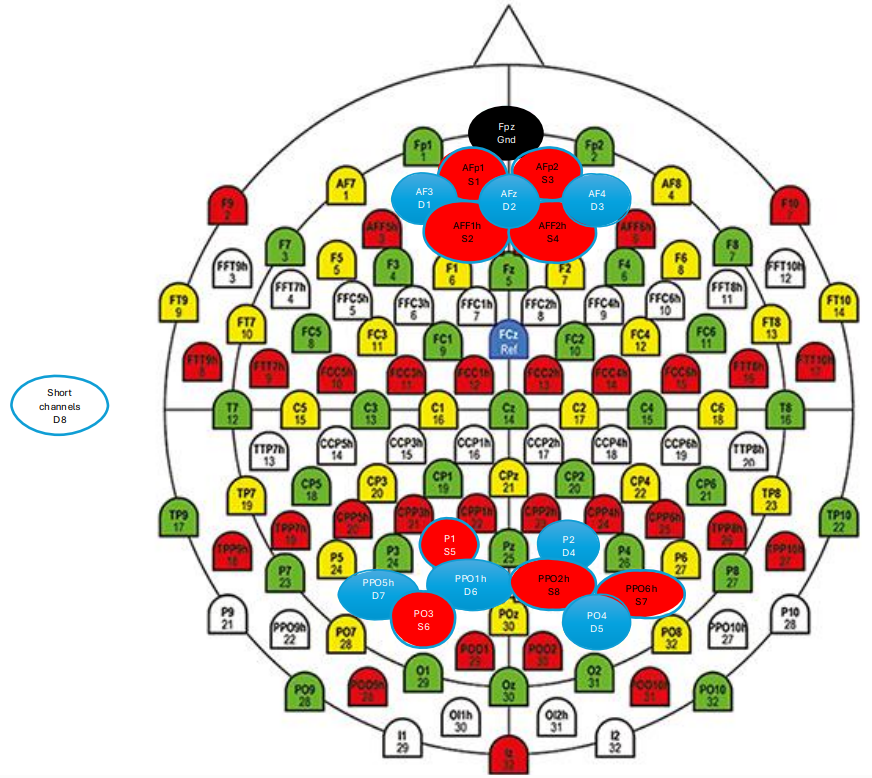
\includegraphics[width=0.48\textwidth]{../EV_images/EV_cogMeasSetupMod.png} % Include setup image (adjust path/size)
    \caption{Placement Setup for Simultaneous \gls{EEG} and \gls{fNIRS}.}
    \label{fig:eegsetup} % Label for referencing
    \parbox{0.8\textwidth}{\scriptsize Combined \gls{EEG}/\gls{fNIRS} setup. Blue = detectors, Red = sources. Circled sources connect to short channel detectors.} % Detailed description
\end{figure}

\subsection{Experimental Design}
This study utilized a within-subjects design, where each participant was exposed to all experimental conditions, allowing for control of inter-individual variability. Stimuli were presented, and behavioral responses recorded, using PsychoPy (v[e.g., 2022.2.5]) \parencite{peircePsychoPyPsychophysicsSoftware2007, peircePsychoPy2BuilderCoder2019} running on a standard laboratory computer with a [e.g., 24-inch] monitor, viewed from a distance of approximately [e.g., 60 cm]. Participants viewed emotionally evocative video clips intended to induce distinct affective states: positive, negative, or neutral. A total of nine unique video clips (three per valence category: positive, negative, neutral) were selected from the E-MOVIE database \parencite{maffeiEMOVIEExperimentalMOVies2019}. Clip durations ranged from [e.g., 60] to [e.g., 180] seconds (M = [e.g., 120], SD = [e.g., 30]). This database was chosen, as highlighted in the introduction, due to its validated effectiveness in reliably eliciting targeted emotional responses and its provision of normative ratings for valence and arousal, ensuring robust emotional induction. The selected clips were translated into German for use with native German-speaking participants. To manage stimulus presentation and minimize potential order effects (e.g., carry-over of emotional state from one clip to the next), three bundles of video clips were created. Each bundle contained one randomly ordered scene of each valence (positive, negative, neutral). The presentation order of these three bundles was counterbalanced across participants using a [e.g., Latin square design or simple permutation scheme]. An additional constraint was applied such that the valence of the last scene in one bundle differed from the valence of the first scene of the immediately subsequent bundle to further mitigate carry-over effects.

Before the task, participants completed baseline questionnaires, including the German version of the \gls{BIS}/\gls{BAS} scales ([e.g., 20 items for BAS, 7 items for BIS], rated on a [e.g., 4]-point Likert scale ranging from "strongly agree" to "strongly disagree") \parencite{carverBehavioralInhibitionBehavioral1994, strobelDeutschsprachigeVersionBIS2006} to assess trait motivational tendencies, and the German version of the \gls{PANAS} ([e.g., 20 items, 10 for positive and 10 for negative affect], rated on a [e.g., 5]-point Likert scale indicating the extent to which they felt each emotion "right now") \parencite{watsonDevelopmentValidationBrief1988,breyerDeutscheVersionPositive2016} to assess current affective state. The experimental procedure involved repeating a specific trial structure nine times (once for each of the nine scenes). Each trial consisted of: a 1-minute baseline rest period (participants were instructed to relax, minimize movement, and look at a white fixation cross presented on a grey background on the screen, allowing physiological measures to stabilize), presentation of the video clip (audio was delivered via headphones at a comfortable listening level), a 2-minute recovery rest period (fixation cross, to allow physiological responses to return towards baseline), and completion of post-stimulus questionnaires (\gls{SAM} for valence and arousal, emotional adjectives, basic emotion evaluation, and familiarity rating \parencite{maffeiEMOVIEExperimentalMOVies2019}). The \gls{SAM} scales were presented on the computer, and participants responded using the mouse. Scheduled breaks of approximately [e.g., 5] minutes were provided between bundles, during which participants could rest and were verbally asked about their fatigue levels and comfort. The entire experimental session lasted approximately [e.g., 1.5 to 2] hours, including setup and debriefing.

\subsection{Participants}
A total of [N] participants were recruited for this study from the student population of Ruhr-University Bochum and the local community via online advertisements and flyers. [Detail any exclusions and the final sample size, e.g., "Data from X participants were excluded due to: excessive motion artifacts in the fNIRS data exceeding Y\% of trials (n=A), technical issues with EEG recording resulting in loss of >Z\% of channels (n=B), self-reported failure to follow instructions (n=C), or failure to complete the full session (n=D), resulting in a final sample of N participants (M females, F males; mean age = XX.X years, SD = X.X, range = XX-XX)."] Participants were right-handed (assessed by a condensed version of the Edinburgh Handedness Inventory \parencite{oldfieldAssessmentAnalysisHandedness1971}, requiring a laterality quotient > +40), native German speakers, aged between 18 and 30 years. Screening for inclusion/exclusion criteria was performed via a pre-screening questionnaire and a brief interview on the day of the experiment. Exclusion criteria included any self-reported history of neurological or psychiatric disorders (e.g., epilepsy, major depression, anxiety disorders), current use of psychopharmaceutical medication, cardiovascular conditions, skin allergies or scalp conditions that might impede sensor placement, uncorrected vision or hearing impairments, and prior participation in brain stimulation studies within the last [e.g., 6] months. All participants provided written informed consent prior to their participation and were informed of their right to withdraw at any time without penalty. The study was conducted in a sound-attenuated, dimly lit laboratory room to minimize distractions. The study protocol was approved by the Ethics Committee of the Faculty of Psychology, Ruhr-University Bochum (Approval No. [XXX]) and was conducted in accordance with the Declaration of Helsinki. Participants received [e.g., course credit or €X] as compensation for their time and effort.

\subsection{Data Analysis and Statistics}
All data processing and statistical analyses were conducted using the Python scientific ecosystem (Python version [e.g., 3.9.X]) \parencite{harrisArrayProgrammingNumPy2020, virtanenSciPy10Fundamental2020} on a [Windows/macOS/Linux] operating system. This involved custom scripts that integrated functions from several established open-source libraries, including MNE-Python (version [e.g., 1.X.X]) \parencite{gramfortMEGEEGData2013} for \gls{EEG} processing, NeuroKit2 (version [e.g., 0.2.X]) \parencite{makowskiNeuroKit2PythonToolbox2021} for physiological signal processing (\gls{ECG}, \gls{EDA}), MNE-NIRS (version [e.g., 0.X.X]) \parencite{yucelBestPracticesFNIRS2021} for \gls{fNIRS} analysis, SciPy (version [e.g., 1.7.X]) \parencite{virtanenSciPy10Fundamental2020} for general scientific computing (e.g., filtering, interpolation, Hilbert transform), and `statsmodels` (version [e.g., 0.13.X]) \parencite{seaboldStatsmodelsEconometricStatistical2010} and `pingouin` (version [e.g., 0.5.X]) \parencite{vallatPingouinStatisticsPython2018} for statistical modeling and hypothesis testing. Core aspects of the analysis pipeline, including data synchronization, feature extraction, and integration across modalities, were managed and executed using the custom-developed \href{https://github.com/YourGitHubUser/YourRepoName}{PsyAnalysisToolbox} (version [e.g., 0.1.0]; [If citable, add: \textcite{YourToolboxCitationPlaceholder}]).
The group-level analysis pipeline was orchestrated using the \texttt{GroupAnalyzer} module within the \texttt{PsyAnalysisToolbox}. This module took the processed individual participant artifacts as input and executed a sequence of data aggregation and statistical analysis tasks defined in a configuration file. Data aggregation steps included, but were not limited to, concatenating DataFrames (e.g., trial-wise PLV across participants) and collecting specific metrics (e.g., baseline RMSSD, average FAI, condition-specific EDA metrics) into group-level DataFrames. Statistical analysis tasks then utilized these prepared DataFrames to perform the specified tests via available analyzer modules within the toolbox (e.g., leveraging \texttt{pingouin} for ANOVAs, or \texttt{scipy.stats}/\texttt{pingouin} for correlations). The significance level for all statistical tests was set at $\alpha = 0.05$ (two-tailed, unless otherwise specified for directional hypotheses). Standard assumptions for parametric tests (e.g., normality of residuals via Shapiro-Wilk test, homogeneity of variances via Levene's test, sphericity via Mauchly's test for repeated measures \gls{ANOVA}) were checked. Where assumptions were violated, appropriate corrections (e.g., Greenhouse-Geisser correction for sphericity violations, Welch's t-test for unequal variances) or non-parametric equivalents (e.g., Friedman test for non-normal repeated measures data, Mann-Whitney U test for two independent groups, Spearman's rank correlation for non-normal bivariate data) were applied \parencite{fieldDiscoveringStatisticsUsing2024}. Effect sizes (e.g., partial eta-squared ($\eta_p^2$) for \gls{ANOVA}, Cohen's d for t-tests, Pearson's r or Spearman's $\rho$ for correlations) were reported for all key findings to provide an estimate of the magnitude of the observed effects. Given the multiple hypotheses and comparisons involved, particularly within each work package and for post-hoc tests, the False Discovery Rate (FDR) was controlled using the Benjamini-Hochberg procedure \parencite{benjaminControllingFalseDiscovery1995} applied across relevant families of tests.

% Methods 2.7 (Preprocessing) - Removed Roy citation, shortened last sentence
\paragraph{Preprocessing and Feature Extraction}
Standard and validated preprocessing pipelines were applied to each data modality using the specified Python libraries.

\textbf{\gls{EEG} data} underwent offline preprocessing using MNE-Python. Continuous raw data were first bandpass filtered using a zero-phase [e.g., Butterworth fourth-order] finite impulse response (FIR) filter with cutoffs at [e.g., 0.5 Hz and 40 Hz] to remove slow drifts and high-frequency noise. A notch filter was applied at 50 Hz (and its harmonics at 100 Hz, if necessary) to eliminate power line interference. Data were then re-referenced to [e.g., the average of all electrodes or linked mastoids (TP9/TP10), chosen to provide a stable reference with minimal bias]. Following this, data were segmented into epochs from [e.g., -1000 ms pre-stimulus onset to +X000 ms post-stimulus offset, where X is the duration of the longest video clip plus a buffer of e.g., 2000 ms to capture sustained responses]. [If applicable: Baseline correction was applied to each epoch using the mean signal from a pre-stimulus interval of -Y00 ms to 0 ms, e.g., -500 ms to 0 ms.]
Artifacts such as eye blinks, saccades, and muscle activity were identified and corrected using \gls{ICA} (e.g., Infomax algorithm \parencite{bellIndependentComponentAnalysis1995} or FastICA \parencite{hyvarinenFastRobustFixedPoint1997}) \parencite{delormeEEGLABOpenSource2004}. The number of ICA components was typically set to the rank of the data after bad channel rejection. Components representing artifacts were identified based on their characteristic scalp topography (e.g., frontal for blinks, temporal for muscle), time course, spectral properties (e.g., high power in low frequencies for blinks, broad high-frequency power for muscle), and/or correlation with EOG channels (if recorded separately; otherwise, EOG activity was estimated from bipolar derivations of frontal EEG channels like Fp1-F7 and Fp2-F8). [e.g., "Component classification was aided by the ICLabel algorithm \parencite{pion-tonachiniICLabelAutomatedEEG2019}, and components classified as eye or muscle artifacts with >80\% probability were visually inspected and subsequently removed if deemed artifactual."]
Channels exhibiting excessive noise (e.g., standard deviation exceeding [e.g., 150] µV across the recording) or a flat signal for more than [e.g., 20]\% of the recording duration were identified by visual inspection and interpolated using spherical splines (MNE-Python default). Finally, epochs containing residual artifacts exceeding an absolute voltage threshold of [e.g., ±100 µV] at any non-interpolated channel were rejected prior to further analysis. The average number of retained epochs per condition per participant was [M ± SD, to be filled later].

\textbf{For \gls{ECG} data}, signals were processed using NeuroKit2. Data were bandpass filtered using a [e.g., Butterworth fourth-order] filter with cutoffs at [e.g., 5 Hz and 35 Hz] to enhance R-peak detection while removing baseline wander and muscle artifacts. R-peaks were detected using [specify algorithm, e.g., the Pan-Tompkins algorithm \parencite{panRealTimeQRSDetection1985} as implemented in NeuroKit2, or another validated algorithm like the Hamilton algorithm]. Detected R-peaks were visually inspected for accuracy against the raw \gls{ECG} waveform, and manual corrections (additions or deletions of beat markers) were applied where necessary to correct for missed or misidentified R-peaks. From the corrected R-R intervals (\gls{NN intervals}), \gls{RMSSD} was calculated for baseline periods (e.g., the 1-minute rest before the first trial) and for each experimental trial (see \autoref{eq:rmssd}) \parencite{malikHeartRateVariability1996}. For \gls{PLV} analysis, the discrete \gls{NN intervals} were converted into a continuous instantaneous heart period signal by cubic spline interpolation, resampled at a fixed rate of 4 Hz, a common approach for time-frequency analyses of \gls{HRV} \parencite{lagunaPowerSpectralDensity1998}.

\textbf{\gls{EDA} signals} were processed using NeuroKit2. Data were [e.g., low-pass filtered using a Butterworth second-order filter with a 1 Hz cutoff] to remove high-frequency noise and artifacts. The signal was then decomposed into its tonic (\gls{SCL}) and phasic (\gls{SCR}) components using [specify method, e.g., the cvxEDA algorithm \parencite{benedekDecompositionSkinConductance2010} as implemented in NeuroKit2, using default parameters, which employs a convex optimization approach]. The continuous phasic \gls{SCR} signal, reflecting event-related sympathetic sudomotor responses, was then resampled to 4 Hz using [e.g., linear interpolation] to match the temporal resolution of the interpolated \gls{HRV} signal and facilitate synchronous analysis with \gls{EEG} \parencite{boucseinElectrodermalActivity2012}.

\textbf{\gls{fNIRS} processing} was performed using MNE-NIRS. Raw optical density measurements were first converted to changes in \gls{HbO2} and \gls{HbR} concentrations using the modified Beer-Lambert law, with wavelength-specific differential pathlength factors (DPFs) of [e.g., 6.0 for 760 nm and 5.5 for 850 nm, based on age-appropriate values from literature such as \textcite{scholkmannReviewContinuousWave2014} or \textcite{delpyEstimationOpticalPathlength1988}]. Channels with poor scalp-coupling (e.g., scalp coupling index < [X] or gain > [Y]) were identified and excluded. Motion artifacts, characterized by sharp, high-amplitude spikes in the signal, were identified and corrected using [specify method, e.g., \gls{TDDR} with a threshold of X standard deviations of the signal derivative \parencite{scholkmannReviewContinuousWave2014}, or spline interpolation of affected segments identified by visual inspection and an automated threshold (e.g., signal change > Y µM/s), or targeted motion correction using short-channel regression where short-channel signals showing high correlation (r > 0.7) with long-channel signals were used to regress out superficial signal components \parencite{gagnonShortSeparationChannel2012}]. The resulting concentration data were then bandpass filtered ([e.g., 0.01-0.1 Hz using a Butterworth third-order zero-phase filter]) to isolate the task-related hemodynamic response and remove physiological noise such as cardiac pulsations, respiratory effects, and very slow drifts. Average concentration changes for \gls{HbO2} (the chromophore typically showing a more robust response to neural activity) were calculated relative to a pre-stimulus baseline of [e.g., -2 to 0 seconds] for each trial. Prefrontal \gls{ROI}s (e.g., \gls{DLPFC}, \gls{VMPFC}) were defined based on [specify method, e.g., grouping fNIRS channels overlying specific anatomical regions based on the 10-20 system coordinates of the optodes, corresponding to Brodmann Areas 9, 46 for DLPFC and BA 10, 11 for VMPFC, guided by the AAL atlas \parencite{tzourio-mazoyerAutomatedAnatomicalLabeling2002} and visualized using NIRSite (NIRx Medical Technologies, LLC) or custom plotting tools]. These \gls{fNIRS}-derived activations provided the crucial spatial context for guiding the selection of \gls{EEG} channels in the subsequent synchrony analysis.

% Methods 2.7 (Synchrony/Stats) - Shortened PLV description
\paragraph{Neural-Autonomic Synchrony and Statistical Testing}
Neural-autonomic synchrony was quantified using \gls{PLV} \parencite{lachauxMeasuringPhaseSynchrony1999} between prefrontal \gls{EEG} signals and continuous autonomic signals. \gls{PLV} measures the consistency of the phase difference ($\Delta\phi(t) = \phi_{\text{EEG}}(t) - \phi_{\text{Autonomic}}(t)$) over a specified time window:
\begin{equation}
    \text{PLV} = \left| \frac{1}{N} \sum_{t=1}^{N} \exp(i \cdot \Delta\phi(t)) \right|
    \label{eq:plv} % Added label for PLV
\end{equation}
where $N$ is the number of time points in the window, $i$ is the imaginary unit, and $\phi_{\text{EEG}}(t)$ and $\phi_{\text{Autonomic}}(t)$ are the instantaneous phases of the filtered \gls{EEG} and the respective continuous autonomic signal (derived from \gls{HRV} or \gls{EDA}) at time $t$. For brain-heart (parasympathetic) coupling, the discrete \gls{NN intervals} were interpolated into a continuous signal (e.g., using cubic splines at a sampling rate of 4 Hz, a standard approach \parencite{lagunaPowerSpectralDensity1998, shafferOverviewHeartRate2017}) via `scipy.interpolate` (SciPy version X.X.X) \parencite{virtanenSciPy10Fundamental2020}. For brain-sudomotor (sympathetic) coupling, the continuous phasic \gls{EDA} signal was resampled (e.g., to 4 Hz) to match the sampling rate of the \gls{HRV}-derived signal. Instantaneous phase was extracted from the filtered \gls{EEG} signals (Alpha and Beta bands) and the continuous autonomic signals via the Hilbert transform, implemented in `scipy.signal` \parencite{virtanenSciPy10Fundamental2020}. \gls{PLV} (see \autoref{eq:plv}) was then computed between selected frontal \gls{EEG} channels (e.g., F4/F3, Fp2/Fp1 \parencite{rodriguesMethodsMatterExamination2021}, further refined by \gls{fNIRS} findings as described below) and the continuous \gls{HRV}-derived and phasic \gls{EDA} signals, respectively. The primary analysis window covered the duration of each stimulus presentation, with comparisons made to \gls{PLV} calculated during the pre-stimulus baseline period. Exploratory analyses examined temporal dynamics within the stimulus period [if applicable, describe briefly], and surrogate data testing (e.g., phase shuffling with [N] surrogates \parencite{cohenAnalyzingNeuralTime2014}) was used to assess the statistical significance of \gls{PLV} values against chance levels.

Specific statistical tests will address the hypotheses:
\begin{enumerate}[label=(\alph*)]
    \item \textbf{\gls{WP}1: \emph{Emotional Modulation of Synchrony}.} As part of the automated group analysis pipeline orchestrated by the \texttt{GroupAnalyzer}, \gls{fNIRS} \gls{HbO2} data were first analyzed using a subject-level \gls{GLM} approach (implemented via MNE-NIRS). The GLM included regressors for each emotional condition, convolved with a canonical hemodynamic response function. Contrasts comparing emotional versus neutral conditions were defined \parencite{yucelBestPracticesFNIRS2021}, and group-level analyses on these contrasts identified functionally relevant prefrontal \gls{ROI}s. \gls{EEG} channels spatially corresponding to these \gls{fNIRS}-defined \gls{ROI}s were then selected for the primary synchrony analysis \parencite{gramfortMEGEEGData2013}. The primary test for emotional modulation of synchrony involved a repeated measures \gls{ANOVA} on the \gls{PLV} values (calculated separately for \gls{EEG}-\gls{HRV} and \gls{EEG}-\gls{EDA} synchrony, and for Alpha and Beta \gls{EEG} bands) derived from these selected \gls{EEG} channels. The \gls{ANOVA} included Emotion (Positive, Negative, Neutral) as the within-subjects factor. Significant main effects of Emotion were followed by FDR-corrected post-hoc pairwise comparisons. This integrated approach, managed by the \texttt{GroupAnalyzer}, ensured that the synchrony analysis focused on functionally relevant cortical areas.
    \item \textbf{\gls{WP}2: \emph{Synchrony and Subjective Arousal}.} Pearson correlations were computed to assess the relationship between subjective arousal ratings (obtained via the \gls{SAM}) and the corresponding trial's \gls{PLV} magnitudes (\gls{EEG}-\gls{HRV} and \gls{EEG}-\gls{EDA} from the functionally defined channels/\gls{ROI}s), specifically within the positive and negative emotional conditions.
    \item \textbf{\gls{WP}3: \emph{Baseline Vagal Tone and Task-Related Synchrony}.} A Pearson correlation (or Spearman's $\rho$) was used to assess the relationship between individual differences in resting-state \gls{RMSSD} (representing baseline parasympathetic tone, calculated from the [e.g., 1-minute baseline period preceding the first experimental trial, or the average of all pre-stimulus baseline periods across trials]) and the average \gls{EEG}-\gls{HRV} \gls{PLV} (Alpha and Beta bands) observed during the processing of negative emotional stimuli (using \gls{PLV} from the functionally defined channels/\gls{ROI}s).
    \item \textbf{\gls{WP}4: \emph{Frontal Asymmetry and Branch-Specific Synchrony}.} Frontal asymmetry was quantified using the \gls{FAI}, calculated from alpha band (8-13 Hz) power differences between homologous frontal electrode pairs (e.g., F4/F3, and Fp2/Fp1, selected based on their common use in asymmetry research \parencite{rodriguesMethodsMatterExamination2021, allenIssuesAssumptionsRoad2004}). Alpha power for each selected electrode was computed using Welch's periodogram method with [e.g., 2-second] Hamming windows and [e.g., 50\%] overlap, applied to the EEG data from the stimulus presentation period of each trial. The formula for \gls{FAI} was:
    \begin{equation}
        \text{FAI} = \ln(P_{\text{Right}}) - \ln(P_{\text{Left}})
        \label{eq:fai} % Label for FAI equation
    \end{equation}
    where $P_{\text{Right}}$ and $P_{\text{Left}}$ represent the alpha band power spectral density at homologous right and left frontal electrode sites, respectively (e.g., $P_{\text{F4}}$ and $P_{\text{F3}}$). Exploratory Pearson correlations were then conducted to test for associations between this \gls{FAI} and the strength of \gls{EEG}-\gls{HRV} \gls{PLV} versus \gls{EEG}-\gls{EDA} \gls{PLV} (from functionally defined channels/\gls{ROI}s), particularly during emotional conditions, to investigate potential differential links between cortical motivational direction and coupling with specific autonomic branches.
\end{enumerate}      % Your methods section (assuming it's in the same EV_thesis folder)
% \include{results}       % Example: create results.tex
% \include{discussion}    % Example: create discussion.tex
% \include{conclusion}    % Example: create conclusion.tex

\newpage
\addcontentsline{toc}{section}{References} % Add "References" to the ToC
\printbibliography % Print bibliography

\end{document}